\begin{name}
	{\tenchude}
	{\tendethi}
	{THPT số 1 Tuy Phước}
	{\thoigian}
\end{name}
\Opensolutionfile{ans}[ans/ans-2-TT-ChuyenDH-Vinh-L1-NH21-22]
\begin{ex}%[2D1Y4-1]%4
TCĐ của đồ thị của hàm số $y=\dfrac{3x+1}{x-2}$ là
\choice
{$y=2$}
{$y=3$}
{\True $x=2$}
{$x=-\dfrac{1}{3}$}
\loigiai{
\begin{itemize}
\item Ta có $\lim\limits_{x \to 2^{-}} f(x)=-\infty$.
\item $\lim\limits_{x \to 2^{+}} f(x)=+\infty$.
\end{itemize}
Suy ra TCĐ của đồ thị của hàm số $y=\dfrac{3x+1}{x-2}$ là $x=2$.
}
\end{ex}

\begin{ex}%[2D1Y4-1]%3
TCN của đồ thị của hàm số $y=\dfrac{2x-1}{x+1}$ là
\choice
{$y=-2$}
{\True $y=2$}
{$y=1$}
{$x=-1$}
\loigiai{Ta có $\lim\limits_{x \to \pm\infty} f(x)=\lim\limits_{x \to \pm\infty} \dfrac{2x-1}{x+1}=2$ nên TCN của đồ thị của hàm số $y=\dfrac{2x-1}{x+1}$ là $y=2$.
}
\end{ex}

\begin{ex}%[2D1Y4-1]%1
Nhận xét đúng về các đường tiệm cận ngang của đồ thị $\left(C\right)$ của hàm số $y=f(x)$ là
\choice
{\True  Đường tiệm cận ngang có thể cắt đồ thị $C$}
{Đường tiệm cận ngang không có điểm chung với đồ thị $C$}
{Đồ thị $\left(C\right)$ có tối đa ba đường tiệm cận ngang}
{Đồ thị $\left(C\right)$ luôn có đúng một đường tiệm cận ngang}
\loigiai{
\begin{itemize}
\item Hình vẽ minh họa của đồ thị $(C)$ có thể cắt đường TCN của nó.
\begin{center}
\begin{tikzpicture}[scale=.7,>=stealth, font=\footnotesize, line join=round, line cap=round]
\def\a{1} \def\b{0} \def\c{-2} \def\d{2.5} % Hệ số
\def\xmin{-4} \def\xmax{4}
\def\ymin{-2} \def\ymax{4}
%		\draw[color=gray!50,dashed] (\xmin,\ymin) grid (\xmax,\ymax);
\draw (-3,1)--(3,1)node[above]{{TCN}};
\draw[->] (\xmin,0)--(\xmax,0) node [below]{$x$};
\draw[->] (0,\ymin)--(0,\ymax) node [left]{$y$};
\node at (0,0) [below left]{$O$};
\node at (-2,-1) [below left]{$(C)$};
\draw (-1.7,1)node [below left]{Điểm chung} circle (2pt);
\clip (\xmin+0.1,\ymin+0.1) rectangle (\xmax-0.5,\ymax-0.1);
\draw[smooth,samples=300][domain=-3:1] plot(\x,{\a*(\x)^3+\b*(\x)^2+\c*(\x)+\d});
\end{tikzpicture}
\end{center}
\item Đường tiệm cận ngang có thể cắt đồ thị $C$ đúng nên Đường tiệm cận ngang không có điểm chung với đồ thị $C$ sai.
\item Đồ thị $\left(C\right)$ có tối đa ba đường tiệm cận ngang và Đồ thị $\left(C\right)$ luôn có đúng một đường tiệm cận ngang sai như sau
\item Đồ thị $(C)$ luôn chỉ có tối đa hai đường TCN vì chỉ có tối đa hai giá trị giới hạn hữu hạn khác nhau ở tại vô cực.
\item Đồ thị $(C)$ có thể có tối đa hai đường TCN hoặc không có đường TCN nào nên đồ thị $\left(C\right)$ luôn có đúng một đường tiệm cận ngang là sai.
\end{itemize}
}
\end{ex}

\begin{ex}%[2D1B4-1]%8
Số tiệm cận đứng của đồ thị hàm số $y=\tan x$ là
\choice
{$1$}
{$2$}
{\True vô số }
{$0$}
\loigiai{
Khi $x\to \left(\dfrac{\pi}{2}+k\pi\right)$ thì $y\to \pm \infty$. Suy ra đồ thị hàm số $\tan x$ có vô số đường TCĐ.
}
\end{ex}

\begin{ex}%[2D1B4-1]%9
Số tiệm cận ngang của đồ thị hàm số $y=\tan x$ là
\choice
{\True $0$}
{vô số }
{$1$}
{$3$}
\loigiai{
Khi $x\to \pm \infty$ thì các hàm lượng giác của $x$ không tồn tại giới hạn. Suy ra đồ thị hàm số $\tan x$ không có TCN.
}
\end{ex}

\begin{ex}%[2D1K4-1]%5
Đồ thị của hàm số $y=\sin \dfrac{x}{x^2-1}$ có đường
\choice
{Tiệm cận đứng $x=0$}
{\True Tiệm cận ngang $y=0$}
{Tiệm cận đứng $x=-1$}
{Tiệm cận ngang $y=+\infty$}
\loigiai{
\begin{itemize}
\item Xét $\lim\limits_{x \to \pm\infty} f(x)=\lim\limits_{x \to \pm\infty} \sin \dfrac{x}{x^2-1}=\sin \left(\lim\limits_{x \to \pm\infty} \dfrac{x}{x^2-1}\right)=\sin 0=0$. Suy ra đồ thị hàm số có đúng một đường TCN là $y=0$.
\item Vì $-1\le \sin \dfrac{x}{x^2-1}\le 1 \Rightarrow $ giá trị hàm số không thể tiến đến vô cực. Suy ra không có TCĐ.
\end{itemize}
}
\end{ex}

\begin{ex}%[2D1K4-1]%10
Đồ thị của hàm số $y=\dfrac{\sqrt{2x^2+1}}{x^2+2x+5}$ có số đường tiệm cận ngang là
\choice
{\True $1$}
{$0$}
{$2$}
{$3$}
\loigiai{
Ta có $\lim\limits_{x \to \pm\infty} y=\lim\limits_{x \to \pm\infty} \dfrac{\sqrt{2x^2+1}}{x^2+2x+5}=0 \Rightarrow $ có một đường TCN $y=0$.
}
\end{ex}

\begin{ex}%[2D1K4-1]%11
Đồ thị của hàm số $y=\dfrac{\left|x+1\right|}{2x+5}$ có số đường tiệm cận ngang là
\choice
{$1$}
{\True $2$}
{$3$}
{$0$}
\loigiai{
\begin{itemize}
\item Ta có $\lim\limits_{x \to +\infty} y=\lim\limits_{x \to +\infty}\dfrac{\left|x+1\right|}{2x+5}=\lim\limits_{x \to +\infty}=\lim\limits_{x \to +\infty}=\lim\limits_{x \to +\infty}=\dfrac{1}{2}$.
\item Suy ra ta có TCN $y=\dfrac{1}{2}$ khi $x\to +\infty$.
\item Ta có $\lim\limits_{x \to +\infty} y=\lim\limits_{x \to +\infty}\dfrac{\left|x+1\right|}{2x+5}=\lim\limits_{x \to +\infty}=\lim\limits_{x \to +\infty}=\lim\limits_{x \to +\infty}=\dfrac{1}{2}$.
\item Suy ra ta có TCN $y=-\dfrac{1}{2}$ khi $x\to -\infty$.
\item Suy ra đồ thị hàm số có hai TCN là $y=\pm \dfrac{1}{2}$.
\end{itemize}
}
\end{ex}

\begin{ex}%[2D1K4-1]%12
Tổng số tất cả các đường tiệm cận đứng và tiệm cận ngang của đồ thị của hàm số $y=\dfrac{\sqrt{3x+1}-2}{x^2-1}$ là
\choice
{$2$}
{$3$}
{\True $1$}
{$0$}
\loigiai{
\begin{itemize}
\item Ta có $\colon \lim\limits_{x \to +\infty} y=\lim\limits_{x \to +\infty}\dfrac{\sqrt{3x+1}-2}{x^2-1}  =0$. Suy ra có TCN $y=0$ khi $x\to +\infty$.
\item Mặc dù mẫu số $x^2-1=0 \Leftrightarrow x=\pm 1$, nhưng $x$ không thể tiến đến $x=-1$ được vì tập xác định của hàm số là $\mathscr{D}=\left[ -\dfrac{1}{3};+\infty\right)\setminus \{1\}$.
\item Ta có $\lim\limits_{x \to 1} y=\lim\limits_{x \to 1}\dfrac{\sqrt{3x+1}-2}{x^2-1}=\lim\limits_{x \to 1}\dfrac{3}{\left(x+1\right)\left(\sqrt{3x+1}+2\right)}=\dfrac{3}{8}$.
\item Suy ra ta có TCĐ $x=1$. Suy ra đồ thị hàm số chỉ có $1$ đường tiệm cận.
\end{itemize}
}
\end{ex}

\begin{ex}%[2D1K4-1]%13
Cho hàm số $y=x-\sqrt{x^2+1}$. Mệnh đề nhận xét đúng khi nói về tiệm cận của đồ thị hàm số là
\choice
{\True Hàm số có tiệm cận ngang là trục hoành}
{Hàm số không có tiệm cận nào}
{Hàm số có tiệm cận ngang là $y=1$}
{Hàm số có tiệm cận đứng $x=1$}
\loigiai{
\begin{itemize}
\item Ta có $\colon \lim\limits_{x \to +\infty} y=\lim\limits_{x \to +\infty}\left(x-\sqrt{x^2+1}\right)=\lim\limits_{x \to +\infty}\dfrac{x^2-x^2-1}{\sqrt{x^2+1}+x}=\lim\limits_{x \to +\infty}\dfrac{-1}{x+\sqrt{x^2+1}}=0$
\item Suy ra có TCN  $y=0$ khi $x\to +\infty$.
\end{itemize}
}
\end{ex}

\begin{ex}%[2D1K4-2]%
Cho hàm số $y=\dfrac{mx+1}{x+3n+1}$ có đồ thị $(C)$. Biết đồ thị $(C)$ nhận hai trục tọa độ làm hai đường tiệm cận. Khi đó tổng $(m+n)$ bằng
\choice
{$2$}
{\True $-\dfrac{1}{3}$}
{$\dfrac{1}{2}$}
{$\dfrac{1}{3}$}
\loigiai{
Vì đồ thị $(C)$ nhận hai trục tọa độ làm hai đường tiệm cận.\\
Suy ra $\heva{&ad-bc=m(3n+1)-1 \neq 0 \\&-3n-1=0 \\& m=0}\Leftrightarrow \heva{&m=0 \\&n=-\dfrac{1}{3}}\Rightarrow(m+n)=-\dfrac{1}{3}.$
}
\end{ex}

\begin{ex}%[2D1K4-2]%
Có bao nhiêu giá trị nguyên của tham số $m \in[-10;10]$ để đồ thị hàm số \break $y=\dfrac{x-2}{\sqrt{x^2+m-1}}$ có $4$ đường tiệm cận?
\choice
{$11$}
{\True $10$}
{$12$}
{$9$}
\loigiai{
Đồ thị hàm số $y=\dfrac{x-2}{\sqrt{x^2+m-1}}$ có $4$ đường tiệm cận khi phương trình mẫu có hai nghiệm phân biệt khác $2$
$\Leftrightarrow \heva{& m-1<0\\&4+m-1\neq 0}\Leftrightarrow\heva{& m<1\\&m\neq-3.}$\\
Suy ra $m\in\{-10 ;-9 ;-8 ;-7 ;-6 ;-5 ;-4 ;-2 ;-1 ; 0\}$. Có $10$ giá trị nguyên $m$ thỏa mãn.
}
\end{ex}

\begin{ex}%[2D1K4-2]%
Để đồ thị của hàm số $y=\dfrac{2022}{x^3-6x^2+2mx-1}$ có ba đường tiệm cận đứng cách đều nhau thì giá trị thực của tham số $m$ nằm trong khoảng nào dưới đây?
\choice
{$(8;9)$}
{$(0;4)$}
{\True $(4;6)$}
{$(6;8)$}
\loigiai{
\textbf{Cách 1}
\begin{itemize}
\item Yêu cầu bài toán $\Leftrightarrow $ phương trình $f(x)=x^3-6x^2+2mx-1=0$ có ba nghiệm phân biệt lập thành cấp số cộng.\\
Suy ra điểm uốn nằm trên trục hoành.
\item Ta có
$ f'(x)=3x^2-12x+2m \Rightarrow f''(x)=6x-12=0$.\\
$f''(x)=0\Rightarrow x=x_{u}=2 \Rightarrow y_{u}=f(2)=4m-17=0 \Rightarrow m=\dfrac{17}{4}$
\item Thử lại $m=\dfrac{17}{4} \Rightarrow f(x)=x^3-6x^2+\dfrac{17}{2} x-1=0 \Leftrightarrow x=2;x=\dfrac{4\pm \sqrt{14}}{2}$ (thoả mãn).
\end{itemize}
\textbf{Cách 2}
\begin{itemize}
\item Yêu cầu bài toán $\Leftrightarrow $ phương trình $f(x)=x^3-6x^2+2mx-1=0$ có ba nghiệm phân biệt lập thành cấp số cộng.
\item Gọi $x_1,x_2,x_3$ là $3$ nghiệm lập thành cấp số cộng của phương trình $f(x)=0$.
\item Ta có $x_1+x_2+x_3=-\dfrac{b}{a}=6\Leftrightarrow 3x_2=6\Leftrightarrow x_2=2$.
\item Thay $x_2=2$ vào phương trình, ta được $f(2)=4m-17=0 \Rightarrow m=\dfrac{17}{4}$.
\item Thử lại $m=\dfrac{17}{4} \Rightarrow f(x)=x^3-6x^2+\dfrac{17}{2} x-1=0 \Leftrightarrow x=2;x=\dfrac{4\pm \sqrt{14}}{2}$ (thoả mãn).
\end{itemize}
}
\end{ex}

\begin{ex}%[2D1K4-2]%
Có tất cả bao nhiêu số nguyên $m$ để đồ thị hàm số $y=\dfrac{2019}{(x^2-2mx+m^2-2m+4)\sqrt{x-1}}$ có ba đường tiệm cận?
\choice
{\True$1$}
{$2$}
{$3$}
{$0$}
\loigiai{Dễ thấy đường thẳng $y=0$ là một đường TCN và $x=1$ là một TCĐ của đồ thị hàm số đã cho. Ta tìm điều kiện của $m$ để đồ thị hàm số có đúng một tiệm cận đứng.
\\Đặt $f(x)=x^2-2mx+m^2-2m-2$.
\\TH1: Phương trình $f(x)=0$ có nghiệm kép lớn hơn $1$.
\\$\Leftrightarrow \heva{&\Delta'=m^2-m^2+2m-4=0\\&-\dfrac{b}{2a}=m>1}\Leftrightarrow \heva{&m=2\\&m>1}\Leftrightarrow m=2 $
\\TH2: Phương trình $f(x)=0$ hai nghiệm phân biệt, trong đó có một nghiệm lớn hơn 1 và một nghiệm bé hơn hoặc bằng 1.
\\$\Leftrightarrow \heva{&\Delta'=m^2-m^2+2m-4>0\\&m+\sqrt{2m-4>1}\\&m-\sqrt{2m-4}\le1} \Leftrightarrow \heva{&m>2\\&m+\sqrt{2m-4}>1\\&m-\sqrt{2m-4}\le1}\Leftrightarrow m\in \emptyset $
}
\end{ex}

\begin{ex}%[2D1B5-1]%
\immini%[thm]
{
Cho hàm số $y=f(x)$ có tập xác định trên $\mathbb{R}$. Có các đồ thị $y=f(x)$ và đạo hàm $y=f'(x)$ được cho là hai trong bốn đồ thị $\left(C_1\right),\left(C_2\right),\left(C_3\right),\left(C_4\right)$ như hình vẽ. Hãy chọn đáp án \textbf{đúng} ?
\choice
{Đường $\left(C_1\right)$ biểu diễn $y=f(x),\left(C_3\right)$ biểu diễn $y=f'(x)$}
{\True Đường $\left(C_4\right)$ biểu diễn $y=f(x),\left(C_2\right)$ biểu diễn $y=f'(x)$}
{Đường $\left(C_4\right)$ biểu diễn $y=f(x),\left(C_1\right)$ biểu diễn $y=f'(x)$}
{Đường $\left(C_3\right)$ biểu diễn $y=f(x),\left(C_2\right)$ biểu diễn $y=f'(x)$}
}
{
\begin{tikzpicture}[>=stealth,line join=round,line cap=round,font=\footnotesize,scale=.5]
\draw[->] (0,-2)--(0,5)node[right]{$y$};
\draw[->] (-4.5,0)--(5,0)node[below]{$x$};
\draw (-4,1)--(4,1) node[above]{$(C_2)$};
\draw (-4,2)--(4,2) node[above]{$(C_3)$};
\draw (-4,-1)--(4,-1)node[below]{$(C_1)$};
\draw($(-2,0)!2!(0,2)$)node[above]{$(C_4)$}--($(0,2)!2!(-2,0)$);
\path (0,0)node[above right]{$O$}
(-2,0)node[below]{$-2$}
(0,2)node[above left]{$2$}
;
\end{tikzpicture}
}
\loigiai{Dễ dàng thấy được đường $\left(C_{4}\right)$ là hàm bậc nhất $y=x+2 \Rightarrow y'=1 \Rightarrow$ là đường $\left(C_{2}\right)$.}
\end{ex}

\begin{ex}%[2D1B5-1]%
Cho hàm số $y=f(x)$ có tập xác định trên $\mathbb{R}$. Có các đồ thị $y=f(x)$ và đạo hàm $y=f'(x)$ được cho là hai trong bốn đồ thị $\left(C_1\right),\left(C_2\right),\left(C_3\right),\left(C_4\right)$ như hình vẽ. Hãy chọn đáp \textbf{đúng} ?
\begin{center}
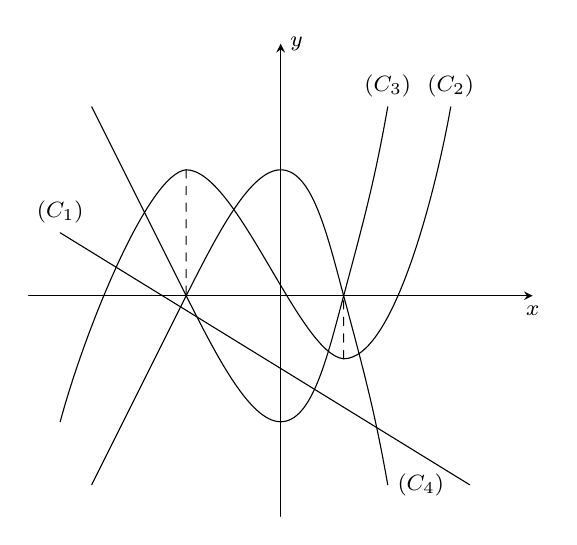
\begin{tikzpicture}[>=stealth,line join=round,line cap=round,font=\footnotesize,scale=.8]
\draw[->] (0,-3.5)--(0,4)node[right]{$y$};
\draw[->] (-4,0)--(4,0)node[below]{$x$};
\path(1,-1) coordinate (A)
(-1.5,2) coordinate (B);
\draw (-3.5,-2)..controls+(75:1.5)and +(185:.6)..(B)..controls+(0:.8)and +(175:.7)..(A)..controls+(0:.8)and +(-100:1.3)..(2.7,3)node[above]{$(C_2)$};
\draw (-3,3)--(-1.5,0)..controls+(-63:1)and +(180:.5)..(0,-2)..controls+(0:.5)and +(-105:1)..(1,0)to[out=75,in=-100](1.7,3)node[above]{$(C_3)$};
\draw (-3,-3)--(-1.5,0)..controls+(63:1)and +(180:.5)..(0,2)..controls+(0:.5)and +(105:1)..(1,0)to[out=-75, in=100](1.7,-3)node[right]{$(C_4)$};
\draw (-3.5,1)node[above]{$(C_1)$}--(3,-3) ;
\draw[dashed] (B)--(-1.5,0) (A)--(1,0);
\end{tikzpicture}
\end{center}
\choice
{Đường $\left(C_1\right)$ biểu diễn $y=f(x),\left(C_3\right)$ biểu diễn $y=f'(x)$}
{\True Đường $\left(C_2\right)$ biểu diễn $y=f(x),\left(C_3\right)$ biều diễn $y=f'(x)$}
{Đường $\left(C_4\right)$ biểu diễn $y=f(x),\left(C_1\right)$ biểu diễn $y=f'(x)$}
{Đường $\left(C_3\right)$ biểu diễn $y=f(x),\left(C_2\right)$ biểu diễn $y=f'(x)$}
\loigiai{Quan sát hình ta thấy
\begin{itemize}
\item Hai đường parabol đi qua gốc $O$ (có cực trị tại điểm 0 ) nếu là hàm $y=f(x) \Rightarrow$ đồ thị đạo hàm là đường thẳng đi qua gốc $O$.\\
Nhưng chỉ có duy nhất một đường thẳng có khả năng là đồ thị đạo hàm thì lại không đi qua gốc $O$. Suy ra không thỏa mãn.
\item Dễ thấy ngay được $\left(C_{2}\right)$ là hàm số $y=f(x)$ và $\left(C_{3}\right)$ là đồ thị đạo hàm tương ứng.
\end{itemize}
}
\end{ex}

\begin{ex}%[2D1B5-1]%
Cho hàm số $y=f(x)$ có tập xác định trên $\mathbb{R}$. Có các đồ thị $y=f(x)$, đạo hàm $y=f'(x)$, đạo hàm cấp hai $y=f''(x)$ được cho là ba trong bốn đồ thị $\left(C_1\right),\left(C_2\right),\left(C_3\right),\left(C_4\right)$ như hình vẽ bên dưới. Hãy chọn đáp án \textbf{đúng} ? $\left(C_1\right)$
\begin{center}
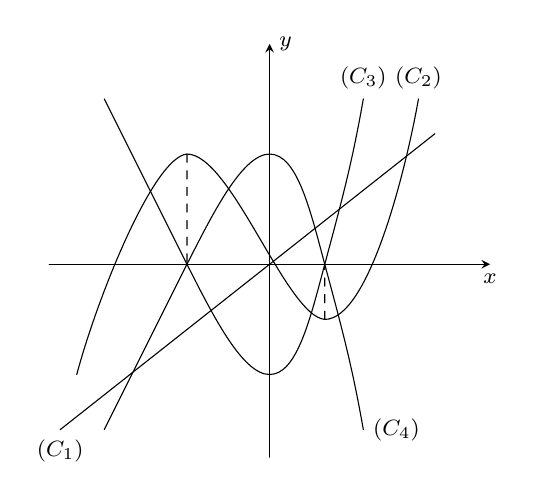
\begin{tikzpicture}[>=stealth,line join=round,line cap=round,font=\footnotesize,scale=.7]
\draw[->] (0,-3.5)--(0,4)node[right]{$y$};
\draw[->] (-4,0)--(4,0)node[below]{$x$};
\path(1,-1) coordinate (A)
(-1.5,2) coordinate (B);
\draw (-3.5,-2)..controls+(75:1.5)and +(185:.6)..(B)..controls+(0:.8)and +(175:.7)..(A)..controls+(0:.8)and +(-100:1.3)..(2.7,3)node[above]{$(C_2)$};
\draw (-3,3)--(-1.5,0)..controls+(-63:1)and +(180:.5)..(0,-2)..controls+(0:.5)and +(-105:1)..(1,0)to[out=75,in=-100](1.7,3)node[above]{$(C_3)$};
\draw (-3,-3)--(-1.5,0)..controls+(63:1)and +(180:.5)..(0,2)..controls+(0:.5)and +(105:1)..(1,0)to[out=-75, in=100](1.7,-3)node[right]{$(C_4)$};
\draw (-3.8,-3)node[below]{$(C_1)$}--(3,2.37) ;
\draw[dashed] (B)--(-1.5,0) (A)--(1,0);
\end{tikzpicture}
\end{center}
\choice
{Đường $\left(C_1\right)$ biểu diễn $y=f(x),\left(C_3\right)$ biểu diễn $y=f'(x),\left(C_2\right)$ biểu diễn $y=f''(x)$}
{Đường $\left(C_4\right)$ biểu diễn $y=f(x),\left(C_2\right)$ biểu diễn $y=f'(x),\left(C_3\right)$ biểu diễn $y=f''(x)$}
{\True Đường $\left(C_2\right)$ biểu diễn $y=f(x),\left(C_3\right)$ biểu diễn $y=f'(x),\left(C_1\right)$ biểu diễn $y=f''(x)$}
{Đường $\left(C_3\right)$ biểu diễn $y=f(x),\left(C_2\right)$ biểu diễn $y=f'(x),\left(C_4\right)$ biểu diễn $y=f''(x)$}
\loigiai{
Chúng ta chỉ cần nắm vững: khi đồ thị hàm số $y=f(x)$ đạt cực trị thì đạo hàm của nó cắt (không tiếp xúc) trục hoành tại đúng điểm đó.\\
Nếu đạt cực đại thì đạo hàm sẽ đi từ trên xuống dưới qua điểm đó. Nếu đạt cực tiểu thì đạo hàm sẽ đi từ dưới lên trên qua điểm đó.\\
Dễ thấy ngay được $\left(C_{2}\right)$ là hàm số $y=f(x)$ và $\left(C_{3}\right)$ là đồ thị đạo hàm $y=f'(x),\left(C_{1}\right)$ là đồ thị của đạo hàm cấp hai $y=f^{\prime \prime}(x)$.
}
\end{ex}

\begin{ex}%[2D1B2-2]%
\immini{
Cho hàm số $y=f(x)$ có đồ thị như hình vẽ. Hãy chọn mệnh đề đúng?
\choice
{Hàm số có tất cả $5$ điểm cực trị}
{\True Hàm số có tất cả $2$ điểm cực tiểu}
{Hàm số có tất cả $3$ điểm cực đại}
{Hàm số có tất cả $2$ điểm cực trị}
}{
\begin{tikzpicture}[scale=0.7,>=stealth, font=\footnotesize, line join=round, line cap=round]
\def\a{-0.41} \def\b{0.85} \def\c{1.41} \def\d{-0.85} % Hệ số
\def\xmin{-4} \def\xmax{6}
\def\ymin{-2} \def\ymax{4}
%	\draw[color=gray!50,dashed] (\xmin,\ymin) grid (\xmax,\ymax);
\draw[->] (\xmin,0)--(\xmax,0) node [below]{$x$};
\draw[->] (0,\ymin)--(0,\ymax) node [left]{$y$};
\node at (0,0) [above left]{$O$};
\clip (\xmin+0.1,\ymin+0.1) rectangle (\xmax-0.5,\ymax-0.1);
\draw[smooth,domain=-2:3,samples=300] plot(\x,{\a*(\x)^3+\b*(\x)^2+\c*(\x)+\d});
\draw (-4,0)--(-2,3) (3,0)--(4,2)--(6,3);
\end{tikzpicture}
}
\loigiai{
Dựa vào đồ thị hàm số, suy ra hàm số có tất cả $2$ điểm cực tiểu.
}
\end{ex}

\begin{ex}%[2D1B2-2]%
\immini{
Cho hàm số $y=f(x)$ có đồ thị như hình vẽ. Hãy chọn đáp án \textbf{sai}?
\choice
{Hàm số có tất cả $3$ điểm cực trị}
{\True Hàm số có duy nhất một điểm cực tiểu}
{Hàm số có $1$ điểm cực đại}
{Đồ thị hàm số có $2$ điểm cực tiểu}
}{
\begin{tikzpicture}[scale=1,>=stealth, font=\footnotesize, line join=round, line cap=round]
\def\a{1} \def\b{-2} \def\c{1} % Hệ số
\def\xmin{-1} \def\xmax{3}
\def\ymin{-1} \def\ymax{2}
%	\draw[color=gray!50,dashed] (\xmin,\ymin) grid (\xmax,\ymax);
\draw[->] (\xmin,0)--(\xmax,0) node [below]{$x$};
\draw[->] (0,\ymin)--(0,\ymax) node [left]{$y$};
\node at (0,0) [below right]{$O$};
\clip (\xmin+0.1,\ymin+0.1) rectangle (\xmax-0.5,\ymax-0.1);
\draw[smooth,domain=-0.6:2.6,samples=300] plot(\x,{\a*(\x-1)^4+\b*(\x-1)^2+\c});
\end{tikzpicture}
}
\loigiai{
Dựa vào đồ thị hàm số, suy ra hàm số có hai điểm cực tiểu.
}
\end{ex}

\begin{ex}%[2D1B2-2]%
\immini{
Cho hàm số $y=f(x)$ liên tục trên toàn $R$ và có đồ thị đạo hàm $y=f'(x)$ như hình vẽ. Mệnh đề nào say đây là đúng?
\choice
{Hàm số có $2$ điểm cực trị}
{Hàm số có $5$ điểm cực trị}
{\True Hàm số có $3$ điểm cực trị}
{Hàm số có $1$ điểm cực trị}
}{
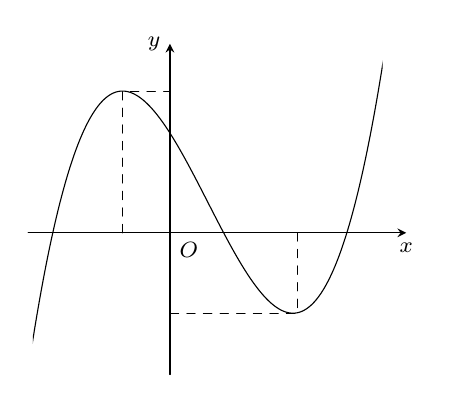
\begin{tikzpicture}[scale=0.6,>=stealth, font=\footnotesize, line join=round, line cap=round]
\def\a{0.2} \def\b{-0.48} \def\c{-1.57} \def\d{2.11} % Hệ số
\def\xmin{-3} \def\xmax{5}
\def\ymin{-3} \def\ymax{4}
%	\draw[color=gray!50,dashed] (\xmin,\ymin) grid (\xmax,\ymax);
\draw[->] (\xmin,0)--(\xmax,0) node [below]{$x$};
\draw[->] (0,\ymin)--(0,\ymax) node [left]{$y$};
\node at (0,0) [below right]{$O$};
\clip (\xmin+0.1,\ymin+0.1) rectangle (\xmax-0.5,\ymax-0.1);
\draw[smooth,samples=300] plot(\x,{\a*(\x)^3+\b*(\x)^2+\c*(\x)+\d});
\draw[dashed](2.7,0)|-(0,-1.7)  (-1,0)|-(0,3);
\end{tikzpicture}
}
\loigiai{
Dựa vào đồ thị hàm số $y=f'(x)$, suy ra hàm số $3$ điểm cực trị.
}
\end{ex}

\begin{ex}%[2D1B2-2]%
\immini{
Cho hàm số $y=f(x)$ liên tục trên toàn $\mathbb{R}$ và có đồ thị đạo hàm $y=f'(x)$ như hình vẽ. Số điểm cực trị của hàm số là
\choice
{$4$}
{$3$}
{$2$}
{\True $1$}
}{
\begin{tikzpicture}[scale=0.6,>=stealth, font=\footnotesize, line join=round, line cap=round]
\def\a{1} \def\b{0} \def\c{-3} \def\d{-1} % Hệ số
\def\xmin{-5} \def\xmax{5}
\def\ymin{-2} \def\ymax{5}
%	\draw[color=gray!50,dashed] (\xmin,\ymin) grid (\xmax,\ymax);
\draw[->] (\xmin,0)--(\xmax,0) node [below]{$x$};
\draw[->] (0,\ymin)--(0,\ymax) node [left]{$y$};
\node at (0,0) [below left]{$O$};
\clip (\xmin+0.1,\ymin+0.1) rectangle (\xmax-0.5,\ymax-0.1);
\draw (-4,-1)
.. controls +(88:1) and +(-170:1) .. (-2,3.5)
.. controls +(-40:1) and +(130:1) .. (-1,1)
.. controls +(30:1) and +(170:1) .. (1,4)
.. controls +(-20:1) and +(150:1) .. (3,0)
.. controls +(10:1) and +(-135:1) .. (4.5,3.5);
\end{tikzpicture}
}
\loigiai{
Từ đồ thị hàm số $y=f'(x)$, suy ra hàm số có $1$ điểm cực trị.
}
\end{ex}

\begin{ex}%[2D1B2-2]%
\immini{
Cho hàm số $y=f(x)$ liên tục trên toàn $R$ và có đồ thị đạo hàm $y=f'(x)$ như hình vẽ. Số điểm cực trị của hàm số là
\choice
{$4$}
{\True $3$}
{$2$}
{$1$}
}{
\begin{tikzpicture}[scale=0.6,>=stealth, font=\footnotesize, line join=round, line cap=round]
\def\a{1} \def\b{0} \def\c{-3} \def\d{-1} % Hệ số
\def\xmin{-5} \def\xmax{5}
\def\ymin{-2} \def\ymax{5}
%	\draw[color=gray!50,dashed] (\xmin,\ymin) grid (\xmax,\ymax);
\draw[->] (\xmin,0)--(\xmax,0) node [below]{$x$};
\draw[->] (0,\ymin)--(0,\ymax) node [left]{$y$};
\node at (0,0) [below left]{$O$};
\clip (\xmin+0.1,\ymin+0.1) rectangle (\xmax-0.5,\ymax-0.1);
\draw (-4,-1)
.. controls +(88:1) and +(-170:1) .. (-2,3.5)
.. controls +(-40:1) and +(130:1) .. (-1,0)
.. controls +(30:1) and +(170:1) .. (1,4)
.. controls +(-20:1) and +(150:1) .. (3,-1)
.. controls +(10:1) and +(-135:1) .. (4.5,3.5);
\end{tikzpicture}
}
\loigiai{
Từ đồ thị hàm số $y=f'(x)$, suy ra hàm số có $3$ điểm cực trị.
}
\end{ex}

\begin{ex}%[2D1B2-2]%
\immini{
Cho hàm số $y=f(x)$ liên tục trên toàn $R$ và có đồ thị đạo hàm $y=f'(x)$ như hình vẽ. Mệnh đề nào sau đây là đúng?
\choice
{\True Hàm số có $2$ điểm cực đại và $2$ điểm cực tiểu}
{Hàm số có $3$ điểm cực đại và $2$ điểm cực tiểu}
{Hàm số có $2$ điểm cực đại và $3$ điểm cực tiểu}
{Hàm số có tất cả $6$ điểm cực trị}
}{
\begin{tikzpicture}[scale=0.6,>=stealth, font=\footnotesize, line join=round, line cap=round]
\def\a{1} \def\b{0} \def\c{-3} \def\d{-1} % Hệ số
\def\xmin{-5} \def\xmax{7}
\def\ymin{-3} \def\ymax{5}
%	\draw[color=gray!50,dashed] (\xmin,\ymin) grid (\xmax,\ymax);
\draw[->] (\xmin,0)--(\xmax,0) node [below]{$x$};
\draw[->] (0,\ymin)--(0,\ymax) node [left]{$y$};
\node at (0,0) [below left]{$O$};
\clip (\xmin+0.1,\ymin+0.1) rectangle (\xmax-0.5,\ymax-0.1);
\draw (-4,-1)
.. controls +(88:1) and +(-170:1) .. (-2,3.5)
.. controls +(-40:1) and +(130:1) .. (-1,0)
.. controls +(30:1) and +(170:1) .. (1,4)
.. controls +(-20:1) and +(150:1) .. (3,-1)
.. controls +(10:1) and +(-135:1) .. (4.5,3.5)
.. controls +(-30:1) and +(115:1) .. (6,-2);
\end{tikzpicture}
}
\loigiai{
Dựa vào đồ thị hàm số $y=f'(x)$, suy ra hàm số có $2$ điểm cực đại và $2$ điểm cực tiểu.
}
\end{ex}

\begin{ex}%[2D1B2-2]%
\immini{
Cho hàm số $y=f(x)$ liên tục trên toàn $\mathbb{R}$ và có đồ thị đạo hàm $y=f'(x)$ như hình vẽ. Hỏi hàm số $y=2020 f(x)+2021$ có bao nhiêu điểm cực trị?
\choice
{$2$}
{\True $3$}
{$1$}
{$4$}
}{
\begin{tikzpicture}[yscale=2,xscale=1.5,>=stealth, font=\footnotesize, line join=round, line cap=round]
\def\xmin{-2} \def\xmax{1.5}
\def\ymin{-1} \def\ymax{1}
%	\draw[color=gray!50,dashed] (\xmin,\ymin) grid (\xmax,\ymax);
\draw[->] (\xmin,0)--(\xmax,0) node [below]{$x$};
\draw[->] (0,\ymin)--(0,\ymax) node [left]{$y$};
\node at (0,0) [below right]{$O$};
\clip (\xmin+0.1,\ymin+0.1) rectangle (\xmax-0.5,\ymax-0.1);
\draw[smooth,domain=-0.9:1,samples=300] plot(\x,{2*(\x)^3-(\x))/((\x)+1)+0.2});
\draw[smooth,domain=-2:-1.1,samples=300] plot(\x,{(\x)/((\x)+1)-4});
\draw[dashed] (-1,-2)--(-1,2);
\end{tikzpicture}
}
\loigiai{
Ta có thể gọi một số điểm có giá trị cụ thể trên trục hoành $Ox$.\\
Có đạo hàm $y'=2020f'(x)$.\\
Bảng biến thiên
\begin{center}
\begin{tikzpicture}
\tikzset{double style/.append style={double distance=1.5pt}}
\tkzTabInit[nocadre=true,lgt=1.2,espcl=2.5,deltacl=0.6]
{$x$ /0.6,$y'$ /0.6,$y$ /2}
{$-\infty$,$-3$,$-2$,$-1$,$3$,$+\infty$}
\tkzTabLine{,-,$0$,+,d,-,$0$,+,$0$,+,}
\tkzTabVar{+/$+\infty$,-/CT,+/\text{CĐ},-/CT,R,+/$+\infty$}
\end{tikzpicture}
\end{center}
Suy ra hàm số có hai điểm cực tiểu và một điểm cực đại.
}
\end{ex}

\begin{ex}%[2D1B2-2]%
\immini{
Cho hàm số $y=f(x)$ liên tục trên toàn $\mathbb{R}$ và có đồ thị đạo hàm $y=f'(x)$ như hình vẽ. Hỏi hàm số $y=f(x)$ có bao nhiêu điểm cực trị?
\choice
{$3$}
{$2$}
{\True $1$}
{$0$}
}{
\begin{tikzpicture}[scale=0.7,>=stealth, font=\footnotesize, line join=round, line cap=round]
\def\a{1} \def\b{0} \def\c{-3} \def\d{-1} % Hệ số
\def\xmin{-4.5} \def\xmax{6}
\def\ymin{-4} \def\ymax{4}
%	\draw[color=gray!50,dashed] (\xmin,\ymin) grid (\xmax,\ymax);
\draw[->] (\xmin,0)--(\xmax,0) node [below]{$x$};
\draw[->] (0,\ymin)--(0,\ymax) node [left]{$y$};
\node at (0,0) [below left]{$O$};
\clip (\xmin+0.1,\ymin+0.1) rectangle (\xmax-0.5,\ymax-0.1);
\draw (\xmin,-0.2)
.. controls +(-10:2) and +(110:1) .. (-2.1,-4);
\draw (-1.9,\ymin)
.. controls +(85:1) and +(-160:1) .. (-0.5,3)
.. controls +(-10:1) and +(170:1.5) .. (3,0)
.. controls +(20:1) and +(-110:1) .. (5,4);
%\draw[dashed](-2,0)|-(0,2)  (4,0)|-(0,-2)  (7,0)|-(0,5);
\draw [dashed](-2,\ymin)--(-2,\ymax);
\draw[fill=black]
%(1,0)node[above]{$1$}circle(1pt)
(2,3)node[below right]{$y=f'(x)$}
(3,0)node[below]{$3$}circle(1pt)
(-1,0)node[above]{$-1$}circle(1pt)
(-2,0)node[below left]{$-2$}circle(1pt);
\end{tikzpicture}
}
\loigiai{
Ta có thể gọi một số điểm có giá trị cụ thể trên trục hoành $Ox$.\\
Bảng biến thiên
\begin{center}

\begin{tikzpicture}
\tikzset{double style/.append style={double distance=1.5pt}}
\tkzTabInit[nocadre=true,lgt=1.2,espcl=2.5,deltacl=0.6]
{$x$ /0.6,$y'$ /0.6,$y$ /2}
{$-\infty$,$-2$,$-1$,$3$,$+\infty$}
\tkzTabLine{,-,d,+,$0$,+,$0$,+,}
\tkzTabVar{+/$+\infty$,R,-/\text{CT},R,+/$+\infty$}
\end{tikzpicture}
\end{center}
Suy ra hàm số có đúng một điểm cực tiểu.
}
\end{ex}

\begin{ex}%[2D1B2-2]%
\immini{
Cho hàm số $y=f(x)$ có tập xác định là $\mathscr{D}=\mathbb{R} \backslash\{2\}$ và có đồ thị đạo hàm $y=f'(x)$. Hỏi hàm số $y=f(x)$ có bao nhiêu điểm cực trị?
\choice
{$1$}
{$2$}
{\True $3$}
{$4$}
}{
\begin{tikzpicture}[scale=0.6,>=stealth, font=\footnotesize, line join=round, line cap=round]
\def\a{1} \def\b{0} \def\c{-3} \def\d{-1} % Hệ số
\def\xmin{-4.5} \def\xmax{6}
\def\ymin{-4} \def\ymax{4}
%	\draw[color=gray!50,dashed] (\xmin,\ymin) grid (\xmax,\ymax);
\draw[->] (\xmin,0)--(\xmax,0) node [below]{$x$};
\draw[->] (0,\ymin)--(0,\ymax) node [left]{$y$};
\node at (0,0) [below left]{$O$};
\clip (\xmin+0.1,\ymin+0.1) rectangle (\xmax-0.5,\ymax-0.1);
\draw (-4,-3)
.. controls +(85:1) and +(-170:1) .. (-2,2)
.. controls +(-20:1) and +(155:1) .. (-0.5,-1.5)
.. controls +(15:1) and +(-100:1) .. (1.9,4);
\draw (2.1,-4)
.. controls +(85:1) and +(-160:1) .. (4,0)
.. controls +(-20:1) and +(-120:1) .. (6,-4);
%\draw[dashed](-2,0)|-(0,2)  (4,0)|-(0,-2)  (7,0)|-(0,5);
\draw [dashed](2,\ymin)--(2,\ymax);
\draw[fill=black]
(-3.5,3.5)node[below right]{$y=f'(x)$}
(2,0)node[below right]{$2$}circle(1pt);
\end{tikzpicture}
}
\loigiai{
Ta có thể gọi một số điểm có giá trị cụ thể trên trục hoành $Ox$.\\
Bảng biến thiên
\begin{center}
\begin{tikzpicture}
\tikzset{double style/.append style={double distance=1.5pt}}
\tkzTabInit[nocadre=true,lgt=1.2,espcl=2,deltacl=0.6]
{$x$ /0.6,$y'$ /0.6,$y$ /2}
{$-\infty$,$-4$,$-1$,$1$,$2$,$3$,$+\infty$}
\tkzTabLine{,-,0,+,$0$,-,$0$,+,d,-,$0$,-,}
\tkzTabVar{+/$+\infty$,-/\text{CT},+/\text{CĐ},-/\text{CT},+D+/ /,R,-/$-\infty$}
\end{tikzpicture}
\end{center}
Suy ra hàm số có hai điểm cực tiểu và một điểm cực đại.
}
\end{ex}

\begin{ex}%[Phạm Tuấn]%[2D1B1-2]%
\immini{
Cho hàm số $y=f(x)$ có đồ thị như hình vẽ. Mệnh đề  nào dưới đây đúng?
\choice
{Hàm số nghịch biến trên $\mathbb{R}$}
{Hàm số đồng biến trên $(-3 ;+\infty)$}
{Hàm số đồng biến trên $(-\infty ; 5)$}
{\True Hàm số đồng biến trên $(-6 ;-3)$}
}
{
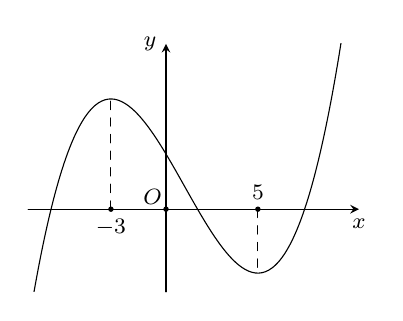
\begin{tikzpicture}[scale=0.7,font=\footnotesize,line join=round, line cap=round,>=stealth]
\draw[->] (-2.5,0)--(3.5,0) node[below]{$x$} ;
\draw[->] (0,-1.5)--(0,3) node[left]{$y$} ;
\draw[fill=black] (0,0) circle(1.1pt) node[above left=-2pt]{$O$} (-1,0) circle(1.1pt) node[below]{$-3$} ({5/3},0)circle(1.1pt)  node[above]{$5$} ;
\draw [dashed] (-1,0)--(-1,2)  ({5/3},0)--({5/3},{-94/81});
\clip (-2.5,-1.5) rectangle (3.5,3) ;
\draw [smooth,samples=100,domain=-2.5:3.5] plot(\x,{(1/3)*((\x)*(\x)*(\x)-(\x)*(\x)-5*(\x))+1}) ;
\end{tikzpicture}
}
\loigiai{
Từ hình vẽ ta thấy hàm số đồng biến trên $(-6 ;-3)$.
}
\end{ex}

\begin{ex}%[Ân Trương]%[2D1B1-2]%
\immini
{
Cho hàm số $y=f(x)$ liên tục trên $\mathbb{R}$ và có đồ thị như hình vẽ. Trong các mệnh đề phát biểu nào dưới đây, hỏi có bao nhiêu mệnh đề phát biểu \textbf{đúng}?
\begin{enumerate}[(1)]
\item Hàm số nghịch biến trên $(-\infty ;-3)$.
\item Hàm số có giá trị không đổi trên đoạn $[-3 ; 4]$.
\item Hàm số đồng biến trên $(-3 ; 4)$.
\item Hàm số nghịch biến trên $(-3 ;+\infty)$.
\item Hàm số nghịch biến trên $[4 ;+\infty)$.
\end{enumerate}
}
{
\begin{tikzpicture}[>=stealth,line join=round,line cap=round,font=\footnotesize,scale=0.5]
\draw[->] (0,-3)--(0,4)node[right]{$y$};
\draw[->] (-6,0)--(10,0)node[below]{$x$};
\path
(0,0) coordinate (O)node[below right]{$ O $}
(1,0) coordinate (O1)
(-3,-1) coordinate (A)
(4,-1) coordinate (B)
;
\draw[dashed](A)--($ (O)!(A)!(O1) $)node[above]{$ -3 $} (B)--($ (O)!(B)!(O1) $)node[above]{$ 4 $};
\draw[blue] ($ (A)+(120:5) $)--(A)--(B)--($ (B)+(-10:6) $)node[above left]{$ f(x) $};
\foreach \i  in{O,A,B} \fill[black] (\i) circle (1.5pt);
\end{tikzpicture}
}
\choice
{$1$}
{$2$}
{\True $3$}
{$4$}
\loigiai{
Dựa vào đồ thị hàm số, mệnh đề đúng là $(1)$; $(2)$ và $(5)$.
}
\end{ex}

\begin{ex}%[Dat Thai, TDM ham so]%[2D1B1-2]%
Cho đồ thị hàm số $y=f(x)$ như hình vẽ.
\begin{center}
\begin{tikzpicture}[line join=round, line cap = round, >=stealth, scale=.8,font=\footnotesize,transform shape]
\foreach \x/\y/\z/\g in
{
0/0/O/-135, -1/0/-1/-45, 1/0/1/-135, 2/0/2/90, 3/0/3/-45
}
\draw[fill=black] (\x,\y) circle(1pt) coordinate (\z) ($(\z)+(\g:3.2mm)$) node{$\z$};
\draw (-2,-2)--(0,2)--(2,-2)--(4,2);
\draw[dashed,fill = black] (0,2) circle(1pt) (2,0)--(2,-2) circle(1pt);
\draw[->] (-2.1,0)--(4.2,0) node[above right]{$x$};
\draw[->] (0,-2.1)--(0,2.3) node[above right]{$y$};
\end{tikzpicture}
\end{center}
Hàm số $y=|f(x)|$ nghịch biến trên khoảng
\choice
{$(0;2)$}
{$(2;+\infty)$}
{\True $(-\infty;-1)$}
{$(-1;1)$}
\loigiai{
Từ đồ thị của hàm số $y=f(x)$ ta thấy bảng biến thiên của hàm số $y=f(x)$ và $y=|f(x)|$ như sau
\begin{center}

\begin{tikzpicture}[scale=1,font=\footnotesize, line join=round, line cap=round, >=stealth, transform shape]
\tkzTabInit[nocadre=false,lgt=1.4,espcl=2,deltacl=0.6]
{$x$ /0.6, $f(x)$ /2, $|f(x)|$ /2}
{$-\infty$,$-1$,$0$,$1$,$2$,$3$,$+\infty$}
\tkzTabVar{-/ , R/ , +/ ,R/,-/,R/,+/} % hàng 3 cột 2 (2 điểm đầu)
\tkzTabIma{1}{3}{2}{$0$} % giữa cột 1 và cột 3
\tkzTabIma{3}{5}{4}{$0$} % giữa cột 3 và cột 5
\tkzTabIma{5}{7}{6}{$0$} % giữa cột 3 và cột 5
\tkzTabVar{+/, -/ $0$ , +/ ,-/$0$,+/,-/ $0$, +/}
\end{tikzpicture}
\end{center}
Do đó hàm số $y=|f(x)|$ nghịch biến trên khoảng $(-\infty;-1)$.
}
\end{ex}

\begin{ex}%[2D1G5-1]% %[Hoang Nguyen]%
\immini{
Cho hàm số trùng phương $y=a x^{4}+b x^2+c$ có đồ thị như hình vẽ bên. Giá trị của biểu thức $(a+b+c)$ nằm trong khoảng
\choice
{\True $(-3;-2)$}
{$(-2;-1)$}
{$(-1; 0)$}
{$(0; 1)$}
}{
\begin{tikzpicture}[>=stealth,line join=round,line cap=round,font=\footnotesize,scale=1]
\draw[->] (-2,0)--(0,0)node[below left]{$O$} --(3,0)node[below]{$x$};
\draw[->] (0,-3.5) -- (0,1) node[right]{$y$};
\draw[smooth] plot[domain=-1.7:1.7] (\x,{(\x)^4-2*(\x)^2-2})node[right]{$(C)$};
\pgfmathsetmacro{\a}{sqrt(sqrt(3)+1)}
\draw[dashed] (1,-3)--(-1,-3);
\foreach \x/\y in {1/-3, -1/-3, 0/-2, \a/0}
\fill (\x,\y) circle (1.2pt);
\path (0,-3) node[below left] {$-3$} (0,-2) node[left] {$-2$} (\a,0) node[below right] {$\sqrt{2}$};
\end{tikzpicture}
}
\loigiai{
Dựa vào đồ thị rõ ràng là ta có $a>0, b<0$.\\
Ta có hệ $\left\{\begin{aligned}&c=-2 \\ &f(\sqrt{2})=4 a+2 b+c=0 \\ &-\dfrac{\Delta}{4 a}=-\dfrac{b^2-4 a c}{4 a}=-\dfrac{b^2}{4 a}+c=-3\end{aligned}\right. \Leftrightarrow\left\{\begin{aligned}&c=-2 \\ &4 a+2 b-2=0 \\ &-\dfrac{b^2}{4 a}-2=-3\Leftrightarrow b^2=4 a \end{aligned}\right.$.\\
Suy ra: $4 a+2 b-2=0 \Leftrightarrow b^2+2 b-2=0 \Leftrightarrow b=-1 \pm \sqrt{3} \stackrel{b<0}{\longrightarrow} b=-1-\sqrt{3}$.\\
Suy ra: $a=\dfrac{b^2}{4}=\dfrac{(-1-\sqrt{3})^2}{4}=\dfrac{2+\sqrt{3}}{2} \Rightarrow(a+b+c)=-2-\dfrac{\sqrt{3}}{2} \approx-2,87$.
}
\end{ex}

\begin{ex}%[2D1G5-1]% %[Hoang Nguyen]%
\immini{
Cho hàm số trùng phương $y=a x^{4}+b x^2+c$ có đồ thị như hình vẽ bên. Giá trị của biểu thức $(a+b+c)$ bằng
\choice
{$46$}
{\True $12$}
{$24$}
{$32$}
}{
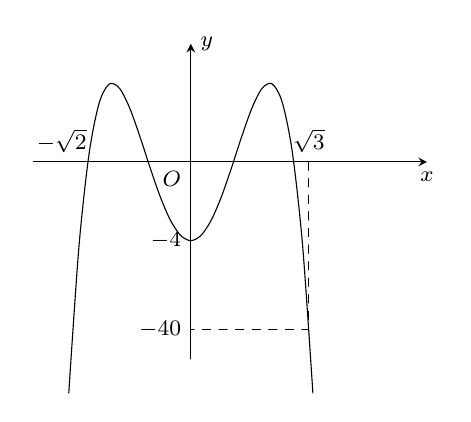
\begin{tikzpicture}[>=stealth,line join=round,line cap=round,font=\footnotesize,scale=1]
\draw[->] (-2,0)--(0,0)node[below left]{$O$} --(3,0)node[below]{$x$};
\draw[->] (0,-2.5) -- (0,1.5) node[right]{$y$};
\pgfmathsetmacro{\a}{1.5}
\pgfmathsetmacro{\b}{-2*(\a)^4+4*(\a)^2-1}
\draw[smooth] plot[domain=-1.55:1.55] (\x,{-2*(\x)^4+4*(\x)^2-1});
\path (-1.2,0) node[above left] {$-\sqrt{2}$} (0,-1) node[left] {$-4$};
\draw[dashed] (\a,0) node[above] {$\sqrt{3}$} |- (0,\b)node[left] {$-40$};
\end{tikzpicture}
}
\loigiai{
Dựa vào đồ thị rõ ràng là ta có $a<0, b>0$.\\
Ta có hệ $\left\{\begin{aligned}&f(0)^2=c=-4 \\ &f(-\sqrt{2})=4 a+2 b+c=0 \\ &f(\sqrt{3})=9 a+3 b+c=-40\end{aligned}\right. \Leftrightarrow\left\{\begin{aligned}&a=-14 \\ &b=30 \\ &c=-4\end{aligned} \Rightarrow(a+b+c)=12.  \right.$
}
\end{ex}

\begin{ex}%[2D1G5-1]% %[Hoang Nguyen]%
\immini{
Cho hàm số trùng phương $y=a x^{4}+b x^2+c$ có đồ thị như hình vẽ bên. Giá trị của biểu thức $\left(a^{3}+b^{3}+c^{3}\right)$ tương ứng bằng
\choice
{\True $56$}
{$72$}
{$24$}
{$16$}
}{
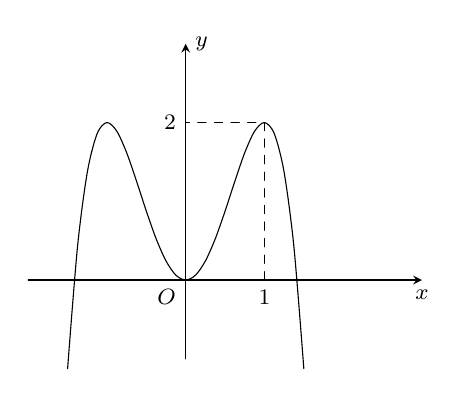
\begin{tikzpicture}[>=stealth,line join=round,line cap=round,font=\footnotesize,scale=1]
\draw[->] (-2,0)--(0,0)node[below left]{$O$} --(3,0)node[below]{$x$};
\draw[->] (0,-1) -- (0,3) node[right]{$y$};
\draw[smooth] plot[domain=-1.5:1.5] (\x,{-2*(\x)^4+4*(\x)^2});
\draw[dashed] (1,0)node[below]{$1$} |- (0,2)node[left]{$2$};
\end{tikzpicture}
}
\loigiai{
Dựa vào đồ thị rõ ràng là ta có $a<0, b>0$.\\
Ta có hệ $\left\{\begin{aligned}&f(0)=c=0 \\ &f'(1)=4 a+2 b=0 \\ &f(1)=a+b+c=2\end{aligned}\right. \Leftrightarrow\left\{\begin{aligned}&a=-2 \\ &b=4 \\ &c=0\end{aligned} \Rightarrow\left(a^{3}+b^{3}+c^{3}\right)=56. \right. $
}
\end{ex}

\begin{ex}%[Ân Trương]%[2D1Y1-2]%
\immini
{
Cho hàm số $ y=f(x) $ có đồ thị đạo hàm $ f'(x) $ như hình vẽ. Mệnh đề phát biểu nào dưới đây \textbf{đúng}?
\choice
{Hàm số nghịch biến trên $(-\infty; -3)$}
{\True Hàm số đồng biến trên $(3; 6)$}
{Hàm số đồng biến trên $(-3; 2)$}
{Hàm số đồng biến trên $(7; +\infty)$}
}
{
\begin{tikzpicture}[>=stealth,line join=round,line cap=round,font=\footnotesize,scale=0.5]
\def\f(#1){-0.1209502917*(#1)^3-0.1881229995*(#1)^2+2.1245674656*(#1)+1.8532371393}
\def\g(#1){-0.1321381363*(#1)^4+2.3447185095*(#1)^3-13.9490198725*(#1)^2+31.7983798339*(#1)-20.0619403347}
\draw[->] (0,-4)--(0,7)node[right]{$y$};
\draw[->] (-6,0)--(9,0)node[below]{$x$};
\draw[blue,thick,samples=70,smooth,domain=-5.5:2] plot (\x,{\f(\x)});
\draw[blue,thick,samples=70,smooth,domain=2:8.3] plot (\x,{\g(\x)})node[above right]{$f'(x)$};
\path
(0,0) coordinate (O)node[below right]{$O$}
(1,0) coordinate (O1)
(-3,{\f(-3)}) coordinate (A)
(2,{\g(2)}) coordinate (B)
(7,{\g(7)}) coordinate (C)
;
\draw[dashed]
(A)--($(O)!(A)!(O1)$)node[above]{$-3$}
(B)--($(O)!(B)!(O1)$)node[below]{$2$}
(C)--($(O)!(C)!(O1)$)node[below]{$7$}
;
\foreach \i in {O,A,B,C} \fill[black] (\i)circle (2.5pt);
\end{tikzpicture}
}
\loigiai{
Dựa vào đồ thị hàm số $ y=f'(x) $ ta có $ f'(x)\geq 0 $ khi $ x \in (3; 6) $ (ứng với phần đồ thị nằm phía trên trục $ Ox $).\\
Vậy hàm số $ y=f(x) $ đồng biến trên $ (3; 6) $.
}
\end{ex}

\begin{ex}%[2D1B5-4]%
Cho hàm số $y=\dfrac{x+3}{x-1}$ có đồ thị $(C)$ và đường thẳng $d\colon y=x-2m$. Hãy tìm tất cả các giá trị thực của $m$ để $(C)$ cắt $d$ tại hai điểm phân biệt?
\choice
{\True $(-\infty;+\infty)$}
{$(-\infty; 1)$}
{$(1;+\infty)$}
{$\varnothing$}
\loigiai{
Xét phương trình hoành độ giao điểm
\allowdisplaybreaks
$\begin{aligned}[t]
&\quad \dfrac{x+3}{x-1}=x-2m\\
&\Leftrightarrow x+3=(x-1)(x-2m),\,\,(x\ne 1)\\
&\Leftrightarrow x^{2}-2(m+1)x+2m-3=0.\quad (1)
\end{aligned}$\\
Để $(C)$ cắt $d$ tại hai điểm phân biệt khi phương trình $(1)$ có hai nghiệm phân biệt khác $1$\\
$\Leftrightarrow \heva{&\Delta'=(m+1)^{2}-2m+3>0\\&1^{2}-2(m+1)\cdot 1+2m-3\ne 0} \Leftrightarrow \heva{&m^{2}+4>0 \,\,\text{luôn đúng}\,\forall m\in\mathbb{R}\\&-4\ne 0 \,\,\text{luôn đúng}.}$\\
Vậy với mọi $m$ thì $(C)$ luôn cắt $d$ tại hai điểm phân biệt.
}
\end{ex}

\begin{ex}%[2D1B5-4]%
Cho hàm số $y=\dfrac{3x+5}{x+2}$ có đồ thị $(C)$ và điểm $A(0; 2)$. Gọi $d$ là đường thẳng đi qua $A$ với hệ số góc là $k$. Số giá trị thực của $k$ để $d$ cắt $(C)$ tại hai điểm phân biệt $A$ và $B$ sao cho độ dài đoạn thẳng $AB=\dfrac{3\sqrt{6}}{2}$ là
\choice
{$3$}
{\True $4$}
{$1$}
{$2$}
\loigiai{
Phương trình đường thẳng $d$ là $y=k(x-0)+2=kx+2$.\\
Xét phương trình hoành độ giao điểm
\allowdisplaybreaks
$\begin{aligned}[t]
&\quad \dfrac{3x+5}{x+2}=kx+2\\
&\Leftrightarrow 3x+5=(x+2)(kx+2),\,\,(x\ne-2)\\
&\Leftrightarrow kx^{2}+(2k-1)x-1=0. \quad (1)
\end{aligned}$\\
Đường thẳng $d$ cắt đồ thị $(C)$ tại $2$ điểm phân biệt khi và chỉ khi phương trình $(1)$ có hai nghiệm phân biệt khác $-2$
$$\Leftrightarrow \heva{&k\neq 0\\&\Delta=(2k-1)^{2}+4k=4k^{2}+1>0\\&k\cdot(-2)^{2}+(2k-1)\cdot(-2)-1\ne 0} \Leftrightarrow k\neq 0. \quad (*)$$
Giao điểm của $d$ và $(C)$ là $A\left(x_{A}; kx_{A}+2\right), B\left(x_{B}; kx_{B}+2\right)$ với $\heva{&x_{A}+x_{B}=-\dfrac{2k-1}{k}\\&x_{A}x_{B}=-\dfrac{1}{k}.}$\\
Ta có
\allowdisplaybreaks
$\begin{aligned}[t]
\dfrac{27}{2}&=AB^2\\
&=\left(x_{A}-x_{B}\right)^{2}+\left(y_{A}-y_{B}\right)^{2}\\
&=\left(x_{A}-x_{B}\right)^{2}+\left(kx_{A}+2-kx_{B}-2\right)^{2}\\
&=\left(k^{2}+1\right)\left(x_{A}-x_{B}\right)^{2}\\
&=\left(k^{2}+1\right)\left(x_{A}-x_{B}\right)^{2}\\
&=\left(k^{2}+1\right)\left[\left(x_{A}+x_{B}\right)^{2}-4x_{A}x_{B}\right]\\
&=\left(k^{2}+1\right)\left[\left(-\dfrac{2k-1}{k}\right)^{2}-4\left(-\dfrac{1}{k}\right)\right]\\
&=\dfrac{\left(k^{2}+1\right)\left(4k^{2}+1\right)}{k^{2}}
\end{aligned}$\\
$\Leftrightarrow \hoac{&k=\pm\sqrt{2}\\&k=\pm\dfrac{1}{2\sqrt{2}}}$ (tmđk $(*)$).
}
\end{ex}

\begin{ex}%[Dự án Tex hóa Tư Duy Mở]%[Nhật Thiện]%[2D1K5-4]%
Cho hàm số $y=f(x)=x^4-8 x^2+7$. Hãy tìm tất cả các giá trị thực của tham số $m$ để phương trình $f(x)=2 m-1$ có bốn nghiệm phân biệt?
\choice
{$m \in(0; 8)$}
{\True $m \in(- 4; 4)$}
{$m \in(4;+\infty)$}
{$m \in\left(- \infty; \dfrac{1}{2}\right)$}
\loigiai{\begin{center}
\begin{tikzpicture}[scale=1, font=\footnotesize, line join=round, line cap=round, >=stealth]
\draw[->] (-2.1,0)--(2.1,0) node[below left] {$x$};
\draw[->] (0,-1.1)--(0,3.1) node[below left] {$y$};
\draw[fill=black] (0,0) circle (1pt) node [below left] {$O$};
\draw[fill=black] (0,1.5) circle (1pt) node [above right] {$A(0;c)$};
\draw[dashed] (-2.1,.5)--(2.1,.5) node[right]{$-\dfrac{\Delta}{4a}$};
\draw (-2.1,1)node[left]{$y=2m-1$}--(2.1,1) ;
\begin{scope}
\clip (-2,-1) rectangle (2,3);
\draw[samples=200,domain=-2:2,smooth,variable=\x] plot (\x,{1*((\x)^4)+0*((\x)^3)-2*((\x)^2)+0*(\x)+1.5});
\end{scope}
\end{tikzpicture}
\end{center}
Để phương trình đã cho có $4$ nghiệm phân biệt thì ta phải có
$$-\dfrac{\Delta}{4a}<2 m-1<c \Leftrightarrow-9<2 m-1<7 \Leftrightarrow-4<m<4.$$
}
\end{ex}

\begin{ex}%[2D1K5-4]%2
Cho hàm số $f(x)=x^3-3x$. Số nghiệm của phương trình $f(x^3-3x^2+1)=2$ là
\choice
{$14$}
{\True $4$}
{$16$}
{$17$}
\loigiai{
\begin{itemize}
\item [Cách 1.]  Với những phương trình ở dạng $f(u)=\alpha$, trong đó số thực $\alpha$ cụ thể thì chúng ta làm trực tiếp luôn cũng rất đơn giản\\
$f(x^3-3x^2+1)=f(u)=u^3-3u=2 \Leftrightarrow \hoac{&u=2=x^3-3x^2+1 &\Rightarrow 1\text{ nghiệm }\\&u=-1=x^3-3x^2+1 &\Rightarrow 3\text{ nghiệm }.\\}$\\
Vậy phương trình $f(x^3-3x^2+1)=2$ có đúng $4$ nghiệm thực $x$.
\item [Cách 2.] Lập bảng biến thiên hàm hợp (còn gọi là kĩ năng ghép trục) như sau\\
Ta có bảng biến thiên của $f(u)=u^3-3u$.
\begin{center}

\begin{tikzpicture}
\tkzTabInit[nocadre=true,lgt=1.2,espcl=2.5,deltacl=0.6]
{$u$/0.6, $f'(u)$/0.6, $f(u)$/2}
{$-\infty$,$-1$,$1$,$+\infty$}
\tkzTabLine{,+,$0$,-,$0$,+,}
\tkzTabVar{-/$-\infty$,+/$-2$,-/$2$,+/$+\infty$}
\end{tikzpicture}
\end{center}
Suy ra bảng biến thiên ghép của hàm hợp $f(x^3-3x^2+1)=f(u)$.
\begin{center}
\begin{tikzpicture}
\tkzTabInit[nocadre=true,lgt=1.6,espcl=1.8,deltacl=0.6]
{$ x $/0.6,$ u'$/0.6,$ u$/2,$u $/0.8,$f(u)$/3.5}
{$ -\infty $,,$0$,,$2$,,,$ +\infty $}
\tkzTabLine{,,+,, $0$ ,,-,,$0$,,+,}
\path
(N12)--(N14)node[pos=0.6](A1){$+\infty$}
(N32)--(N34)node[pos=0.1](A2){$1$}
(N52)--(N54)node[pos=0.6](A3){$-3$}
(N82)--(N84)node[pos=0.1](A4){$+\infty$}

(N12)--(N14)node[pos=0.85](B1){$-\infty$}
(N22)--(N24)node[pos=0.85](B2){$-1$}
(N32)--(N34)node[pos=0.85](B3){$1$}
(N42)--(N44)node[pos=0.85](B4){$-1$}
(N52)--(N54)node[pos=0.85](B5){$-3$}
(N62)--(N64)node[pos=0.85](B6){$-1$}
(N72)--(N74)node[pos=0.85](B7){$1$}
(N82)--(N84)node[pos=0.85](B8){$+\infty$}

(N14)--(N15)node[pos=0.9](C1){$-\infty$}
(N24)--(N25)node[pos=0.3](C2){$2$}
(N34)--(N35)node[pos=0.5](C3){$-2$}
(N44)--(N45)node[pos=0.3](C4){$2$}
(N54)--(N55)node[pos=0.7](C5){$-53$}
(N64)--(N65)node[pos=0.3](C6){$2$}
(N74)--(N75)node[pos=0.5](C7){$-2$}
(N84)--(N85)node[pos=0.1](C8){$+\infty$}

(N54)--(N55)node[pos=0.2](D){$y=2$};
\draw ($ (C2)+(-2.0,0) $)--($ (C6) +(3.5,0)$);
\tikzset{arrow style,shorten >=-2pt}
\draw (A1)->(A2);\draw (A2)->(A3);\draw (A3)->(A4);
\draw [-stealth] ($ (B3)+(-0.1,-0.2) $)--($ (B1) +(-0.1,-0.2)$);
\draw [-stealth] ($ (B5)+(0,-0.2) $)--($ (B3) +(0.2,-0.2)$);
\draw [-stealth] ($ (B5)+(0.2,-0.2) $)--($ (B8) +(0.0,-0.2)$);
\draw (C1)->(C2);\draw (C2)->(C3);\draw (C3)->(C4);\draw (C4)->(C5);\draw (C5)->(C6);\draw (C6)->(C7);	\draw (C7)->(C8);
\end{tikzpicture}
\end{center}
Từ bảng biến thiên ta nhận thấy phương trình $f(u)=2$ có đúng $4$ nghiệm thực $x$.
\end{itemize}
}
\end{ex}

\begin{ex}%[Dự án KSHS - Tư duy mở - Nguyễn Tâm Phục]%[2D1G2-2]%
\immini{Cho đồ thị hàm số $y=f'(x)$ như hình vẽ bên dưới. Số điểm cực trị của hàm số $f(4 \cos x+1)$ trên khoảng $(0 ; 4 \pi)$ là
\choice
{$ 5 $}
{$ 7 $}
{$ 9 $}
{\True $ 11 $}
}{
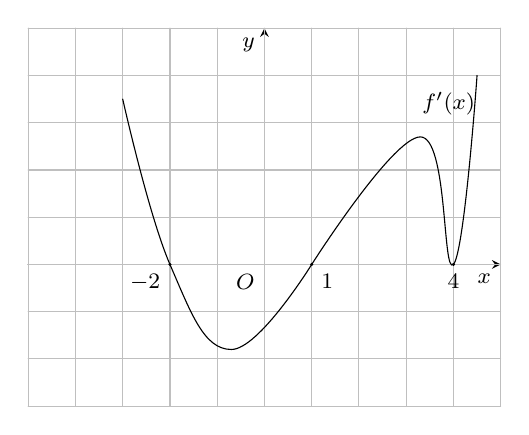
\begin{tikzpicture}[>=stealth,line join=round,line cap=round,font=\footnotesize,scale=0.6]
\def\xmin{-5}
\def\xmax{5}
\def\ymin{-3}
\def\ymax{5}
\tikzset{label style/.style={font=\footnotesize}}
\draw[->] (\xmin,0)--(\xmax,0) node[below left] {$x$};
\draw[->] (0,\ymin)--(0,\ymax) node[below left] {$y$};
\draw (0,0) node [below left] {$O$};
\draw[thin,gray!50,step=1cm] (\xmin,\ymin) grid (\xmax,\ymax);
\begin{scope}
\clip (\xmin,\ymin) rectangle (\xmax,\ymax);
\node (v1) at (-2,0) {};
\node (v2) at (1,0) {};
\node (v3) at (4,0) {};
\draw  plot[smooth, tension=.7] coordinates {(-3,3.5) (v1) (-0.7,-1.8) (v2)};

\draw  plot[smooth, tension=.7] coordinates {(v2) (3.3,2.7) (v3) (4.5,4)};
\node at (3.9,3.4) {$f'(x)$};
\fill (-2,0) node [below left] {$-2$} circle (1pt);
\fill (1,0) node [below right] {$1$} circle (1pt);
\fill (4,0) node [below ] {$4$} circle (1pt);
\end{scope}
\end{tikzpicture}
}
\loigiai
{
Hàm số $f(x)$ đạt cực trị tại $x=-2 ; x=1$. \\
Xét hàm số $f(u)=f(4 \cos x+1)$ trên đoạn $(0 ; 4 \pi)$. \\
Bảng biến thiên của $u=4 \cos x+1$ trên khoảng $(0 ; 4 \pi)$ như sau:
\begin{center}
\begin{tikzpicture}
\tkzTabInit[nocadre=false,espcl=2.5,lgt=1.5]
{$x$/0.7,$u$/3.2}
{$0$,$\pi$,$2\pi$,$3\pi$,$4\pi$}
\tkzTabVar{+/$5$,-/$-3$,+/$5$,-/$-3$,+/$5$}
\node (v1) at (2,-2) {};
\node (v2) at (12,-2) {};
\node (v3) at (2,-3) {};
\node (v4) at (12,-3) {};
\draw (v1) -- (v2);
\draw (v3) -- (v4);
\node [above] at (4.5,-2) {$u=1$};
\node [above] at (7,-3) {$u=-2$};
\end{tikzpicture}
\end{center}
Suy ra $\underset{(0 ; 4 \pi)}{\text{SĐCT}}\{ f(u)\}=\underset{(0 ; 4 \pi)}{\text{SĐCT}}\{u\}+\text{SNBL}\left\{\hoac{&u=1 \\ &u=-2}\right\}=3+8=11$.
}
\end{ex}

\begin{ex}%[Dự án KSHS - Tư duy mở - Nguyễn Tâm Phục]%[2D1G2-2]%
Cho hàm số $f(x)$ có bảng biến thiên như hình vẽ bên dưới. Hỏi có tất cả bao nhiêu giá trị nguyên của tham số $\mathrm{m}$ để số điểm cực trị của hàm số $f\left(x^{3}-3 x+m\right)$ bằng $ 5 $?
\begin{center}
\begin{tikzpicture}
\tkzTabInit[nocadre=false,lgt=1.2,espcl=2,deltacl=0.6]
{$x$/0.6, $f(x)$/3}
{$-\infty$,$-4$,$-3$,$1$,$3$,$+\infty$}
\node [above] (v1) at (1.75,-3.55) {$-\infty$};
\node (v2) at (3.85,-1) {$2$};
\node (v3) at (5.85,-2.3) {$0$};
\node (v4) at (7.8,-2.3) {$0$};
\node (v5) at (9.8,-1.5) {$1$};
\node [above] (v6) at (11.85,-3.6) {$-\infty$};
\draw [-stealth] (v1) -- (v2);
\draw [-stealth] (v2) -- (v3);
\draw [-stealth] (v3) -- (v4);
\draw [-stealth](v4) -- (v5);
\draw [-stealth] (v5) -- (v6);
\end{tikzpicture}
\end{center}
\choice
{\True $3$}
{$ 2 $}
{$ 4 $}
{$ 5 $}
\loigiai
{
Hàm số $f(u)$ đạt cực trị tại $u_{1}=-4, u_{2}=3$, có đạo hàm bằng 0 trên đoạn $[-3 ; 1]$.\\
Xét hàm số $f(u)=f\left(x^{3}-3 x+m\right)$.\\
Ta áp dụng công thức đếm nhanh $\text{SĐCT}$ hàm hợp bất thường như sau:\\
$\text{SĐCT}\{f(u)\}=\text{SĐCT}\{u\}-\text{SĐCT}^{(*)}\{u\}+\text{SNBL}\left\{\hoac{&u=3 \\ &u=-4}\right\}.$ \\
Bảng biến thiên của $u=x^{3}-3 x+m$ như hình vẽ bên dưới:
\begin{center}
\begin{tikzpicture}[>=stealth]
\tkzTabInit[nocadre=false,espcl=2.5,lgt=1.5]
{$x$/0.7,$u'$/0.7,$u$/3}
{$-\infty$,$-1$,$1$,$+\infty$}
\tkzTabLine{,+,0,-,0,+,}
\node (A) at ($ (N13)!0.1!(N12) $) {$ -\infty $};
\node (B) at ($ (N22)!0.2!(N23) $) {$ m+2 $};
\node (C) at ($ (N33)!0.2!(N32) $) {$ m-2 $};
\node (D) at ($ (N43)!0.9!(N42) $) {$ +\infty $};
\draw [->] (A) -- (B);
\draw [->] (B) -- (C);
\draw [->] (C) -- (D);
\node (v1) at (2,-2.7) {};
\node (v2) at (9.5,-2.7) {};
\node (v3) at (2,-3.2) {};
\node (v4) at (9.5,-3.2) {};
\draw (v1) -- (v2)  (v3) -- (v4);
\node [above]at (2.5,-2.5) {$u=3$};
\node [below] at (8.7,-3.2) {$u=-4$};
\end{tikzpicture}
\end{center}
Có $\text{SĐCT}\{u\}=2$ và có $\text{SNBL}\left\{\hoac{&u=3 \\ &u=-4}\right\}=2 k=\{2 ; 4 ; 6\}.$\\
Suy ra
{\allowdisplaybreaks
\begin{eqnarray*}
\text{SĐCT}\{f(u)\}&=&\text{ SĐCT}\{u\}-\text{SĐCT}^{(*)}\{u\}+\text{SNBL}\left\{\hoac{&u=3 \\ &u=-4}\right\}\\
&=&2+2 k-\text{SĐCT}^{(*)}\{u\}=5.
\end{eqnarray*}}
$0 \leq \text{SĐCT}^{(*)}\{u\}=2 k-3 \leq 2 \Leftrightarrow \dfrac{3}{2} \leq k \leq \dfrac{5}{2} \stackrel{k=2}{\Rightarrow}\left\{\hoac{&\text{SNBL}\left\{\hoac{&u=3 \\ &u=-4}\right\}=2 k=4. \\ &\text{SĐCT}^{(*)}\{u\}=1}\right .$\\
Vậy có tất cả $ 3 $ giá trị $m$ nguyên thỏa mãn bài toán.
}
\end{ex}
\Closesolutionfile{ans}